\chapter{Grundlagen}
\label{chapter:grundlagen}

In diesem Kapitel werden die theoretischen und konzeptuellen Grundlagen, die für diese Arbeit von Bedeutung sind, beschrieben. Begonnen wird mit einer kurzen Einführung in das Brettspiel Patchwork, das die Basis dieser Arbeit bildet, indem es spieltheoretisch analysiert und als Computerspiel umgesetzt wird, sowie mit Computergegnern mit künstlicher Intelligenz angereichert wird. Anschließend widmet sich dieses Kapitel der Spieltheorie, einem mathematischen Bereich, der bei der Modellierung und Analyse von Entscheidungssituation verwendet wird, was unter anderem in dem Fall eines Brettspiels zutrifft. Dann wird der Minimax-Algorithmus betrachtet, der ein weit verbreitetes Entscheidungsverfahren in der Spieltheorie und Informatik ist und die grundlegende Theorie von einem der für diese Arbeit implementierten Computergegner darstellt. Anschließend werden die Grundlagen für zwei weitere Computergegner geschaffen, indem die Theorie von \acl{MCTS}, einem heuristischen Suchalgorithmus für Entscheidungsprozesse und AlphaZero, einem Programm, welches durch gegen sich selbst spielen und der Regeln des Brettspiels das Spiel selbstständig erlernt. Abschließend werden interaktive System erläutert, die für die Gestaltung der Benutzerschnittstellen und Spielererfahrung der Computerumsetzung des Brettspiels wichtig sind.

\section{Brettspiel Patchwork}
\label{chapter:brettspiel-patchwork}

\begin{wrapfigure}{r}{0.35\textwidth}
    \centering
    \vspace*{-0.4cm}
    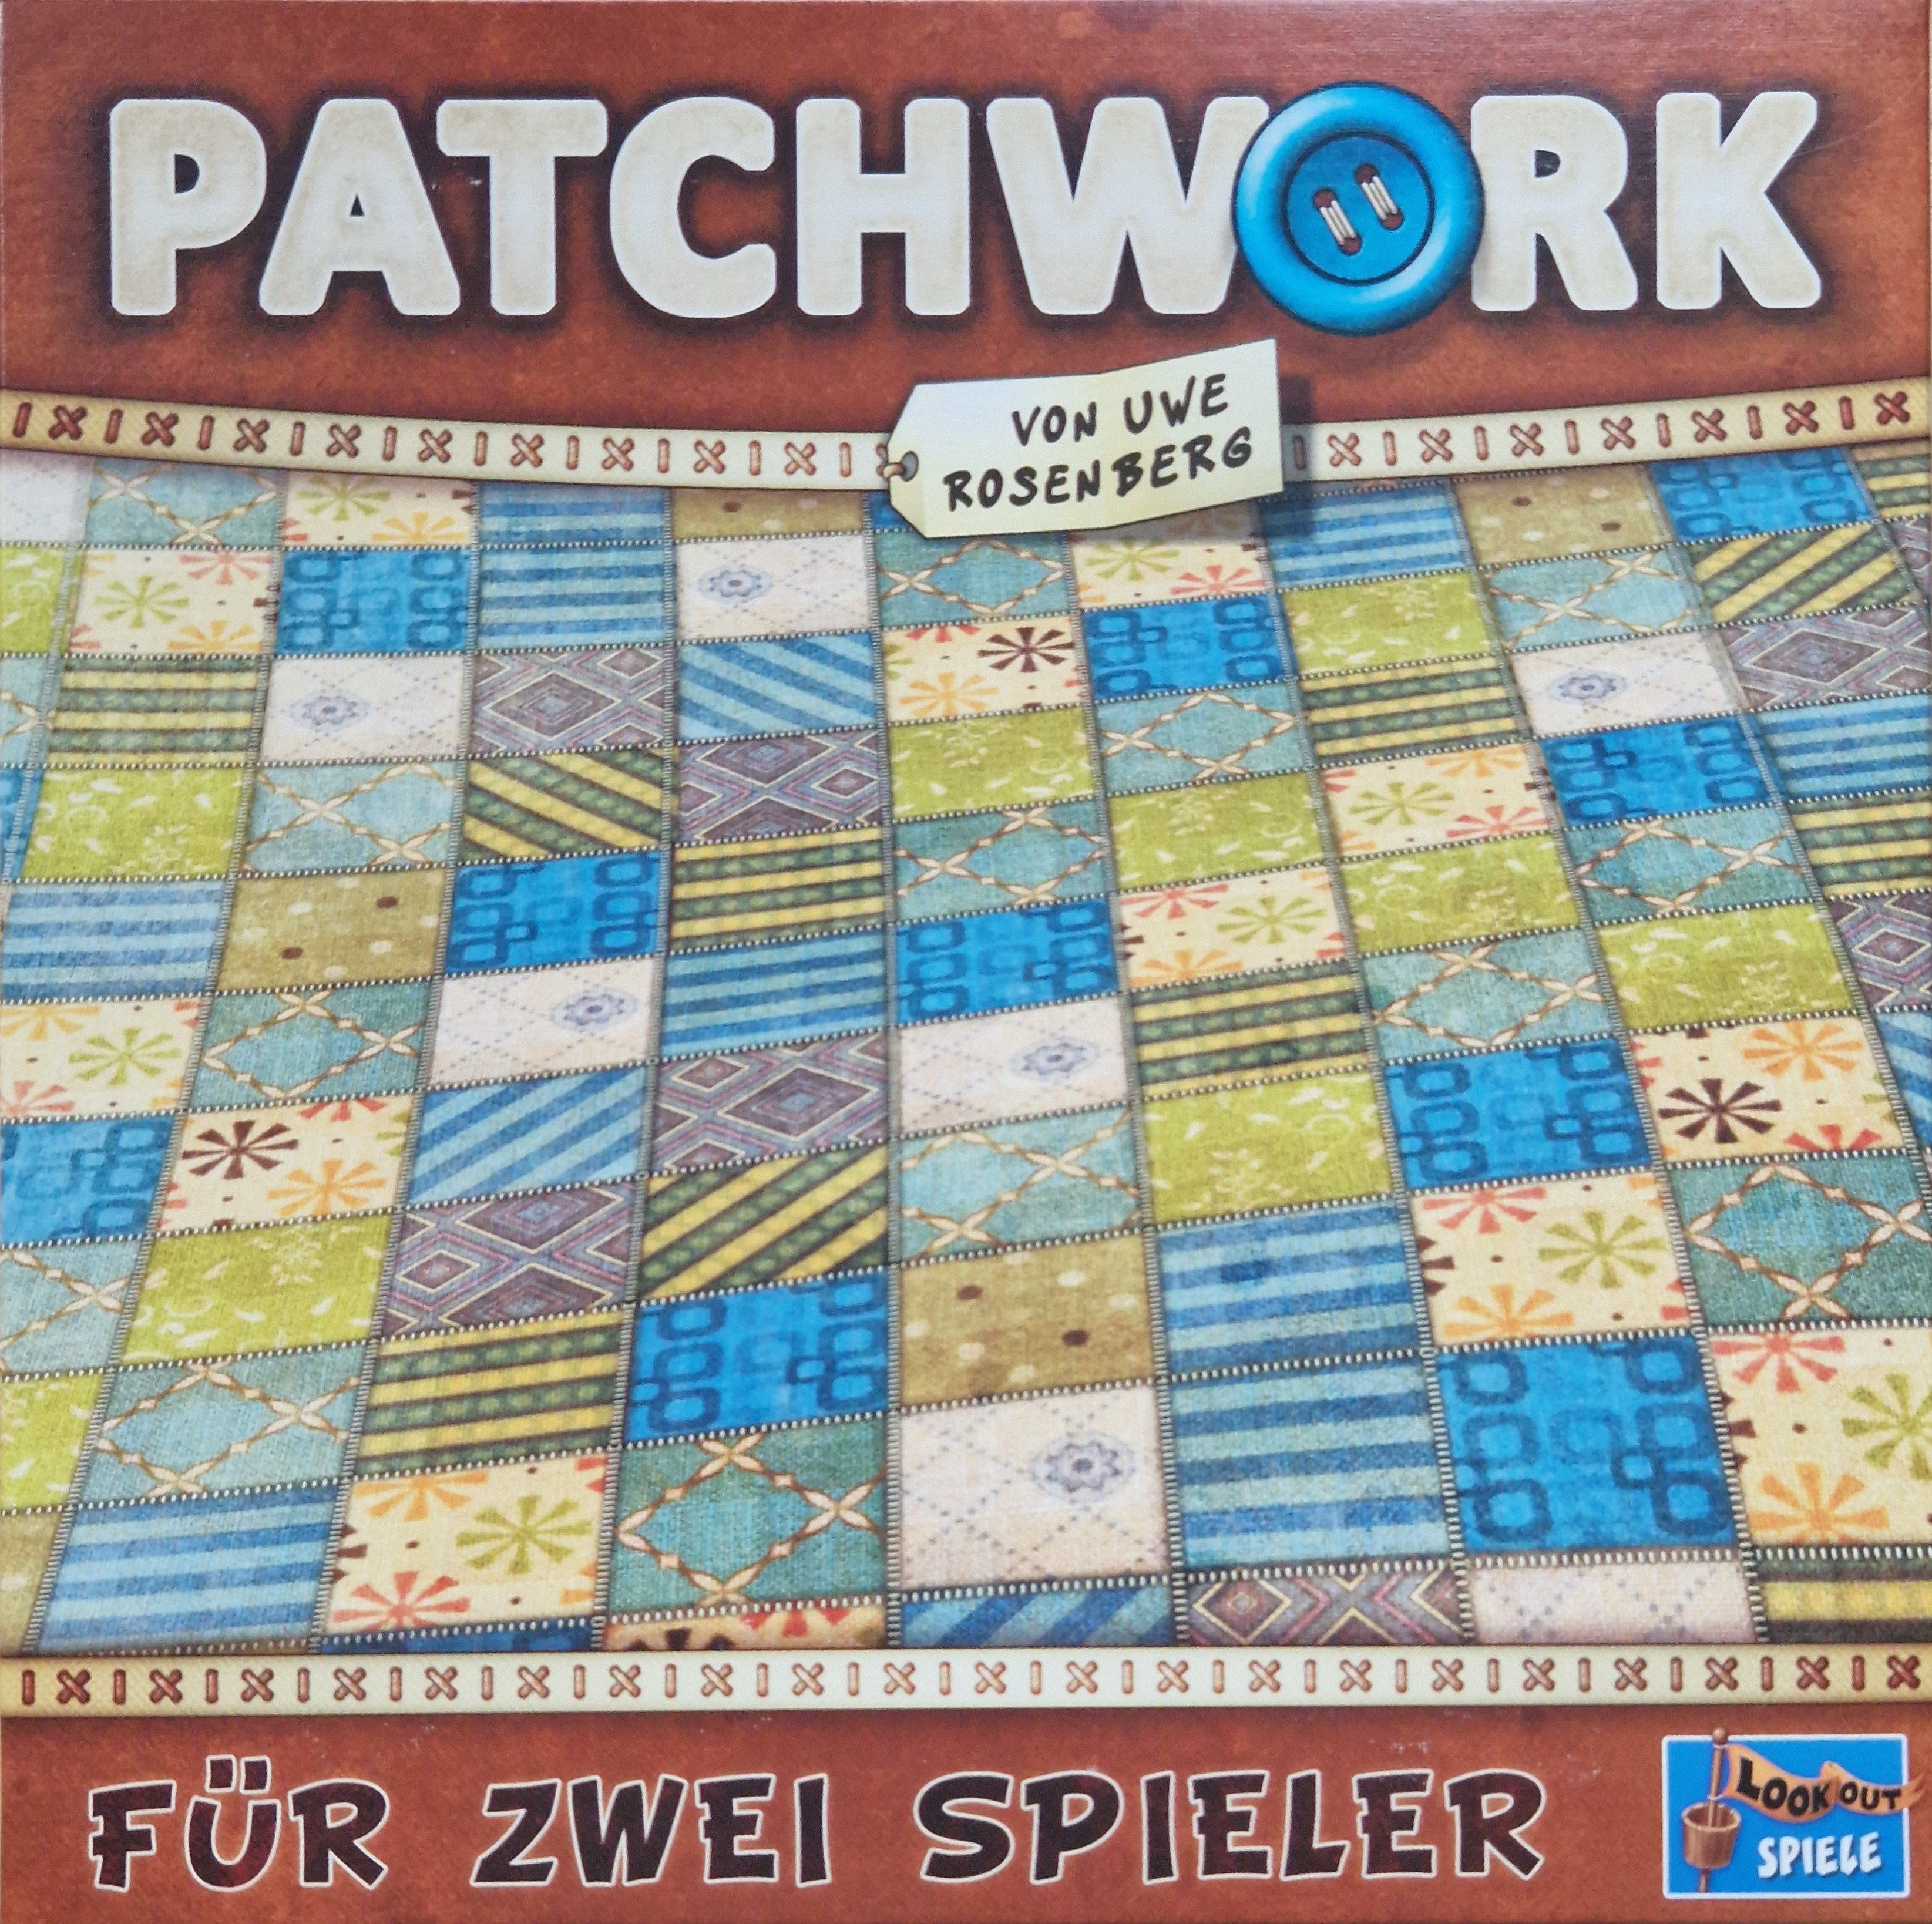
\includegraphics[width=0.3\textwidth]{res/pictures/assets/patchwork-cover.png}
    %\vspace*{-10pt}
    % Das folgende ist ein Trick, um "Abbilgung x.y" in eine
    % eigene Zeile zu packen. Der Text zwischen [ und ] steht
    % im Abbildungsverzeichnis. Der Text darunter wird
    % tatsächlich angezeigt.
    \caption[Cover von Patchwork]{\unskip}
    Cover von Patchwork
    \label{fig:patchwork-cover}
    \vspace*{-2cm}
\end{wrapfigure}


Patchwork ist ein Brettspiel von Uwe Rosenberg, das 2014 bei Lookout Spiele erschienen ist. Bei dem Brettspiel spielen zwei Spieler vom Alter 8 Jahre und aufwärts gegeneinander, wobei ein Spiel in der Regel ungefähr 30 Minuten lang ist. \cite{LookoutSpielePatchwork}

Bei dem Brettspiel gestalten zwei Spieler jeweils eine eigne Decke aus Stoffresten, Flicken und Knöpfen, der Technik entsprechend, die der Titel vorgibt. \cite{SpielDesJahresPatchwork}

Das Ziel der Spieler ist mit den gegebenen Stoffplättchen unterschiedlicher Formen und Größen die vorgegebene Fläche zu füllen. Das Puzzlespiel erfordert taktisches Gespür, da die Flickenauswahl die Zugfolge und auch die Flickenauswahl des Gegenspielers beeinflusst. Immer können die Spieler jedoch nicht die gewünschten Flicken verwenden, da diese mit der Spielwährung Knöpfe aus der eigenen Kasse bezahlt werden müssen. An die begehrten Knöpfe kommen die Spieler über die bereits eingearbeiteten Flicken, welche Knöpfe auf sich abgebildet haben. Je mehr dieser Knöpfe auf der eigenen Decke abgebildet sind, desto höher das Einkommen an Knöpfen. Wer am Schluss des Spiels die meisten Knöpfe erwirtschaftet und seine Decke gut bestickt hat, gewinnt den Nähwettstreit. \cite{SpielDesJahresPatchwork}

\section{Spieltheorie}
\label{chapter:spieltheorie}

TODO:

\subsection{Spielbaum}

TODO: Spielbaum, Entscheidungsbaum

\subsection{Spielkomplexität}

TODO:

\begin{itemize}
    \item \textbf{Zustandsraum-Komplexität}: TODO:
    \item \textbf{Spielbaumgröße}: TODO:
    \item \textbf{Entscheidungskomplexität}: TODO: needed?
    \item \textbf{Spielbaumkomplexität}: TODO:
    \item \textbf{komplexitätstheoretische Rechenaufwand}: TODO: O-Notation $\mathcal{O}(1)$ oder Komplexitätsklasse
\end{itemize}

\section{Minimax-Algorithmus}
\label{chapter:minimax-algorithmus}

TODO:

Hier haben wir mehr

\section{Monte Carlo Tree Search}
\label{chapter:monte-carlo-tree-search}

\begin{equation}
    \mathbb{U}\mathbb{C}\mathbb{T}  \text{UCT} = \frac{w}{n} + c \cdot \sqrt{\frac{\ln N}{n}}
\end{equation}

TODO:

\section{AlphaZero}
\label{chapter:alphazero}

TODO:

\section{Interaktive Systeme}
\label{chapter:interaktive-systeme}

TODO:

